% !TeX root=../main.tex
\chapter{مروری بر مطالعات انجام شده}
%\thispagestyle{empty} 
\section{مقدمه}
در این فصل، پژوهش‌های پیشین در زمینه‌ی موتورهای مسطح مبتنی بر شناوری مغناطیسی (MLPM) با تمرکز بر ویژگی‌های اساسی آنان که به طور کلی در بخش‌های زیر دسته‌بندی شده‌اند، مورد بررسی قرار می‌گیرند. 
\begin{itemize}
	\item
		\textit{معماری دستگاه}:
بررسی انواع معماری‌های موجود برای MLPM و تأثیر آن‌ها بر عملکرد کلی سیستم.
	\item
		\textit{ساختار آهنرباهای دائمی و الکتریکی}:
مرور انواع آهنرباهای الکتریکی و چینش‌های مختلف آهنربا‌های دائمی و نقش آن‌ها در بهینه‌سازی عملکرد سیستم.
	\item
		\textit{طراحی کنترلر}:
معرفی روش‌های کنترل کلاسیک و مدرن برای این سیستم‌ها و چگونگی بهبود پایداری و دقت حرکت.
	\item
		\textit{روش‌های شناسایی سیستم و مدل‌سازی دینامیکی}:
تحلیل روش‌های شناسایی و تخمین مدل‌های دینامیکی سیستم برای شبیه‌سازی و بهینه‌سازی عملکرد.
\end{itemize}
در بخش‌های بعد، پژوهش‌های انجام‌شده بر اساس این ویژگی‌ها ارزیابی شده و مزایا و معایب هر روش مورد بررسی قرار می‌گیرد.

\section{معماری دستگاه‌های MLPM}
سیستم‌های شناوری مغناطیسی به دلیل ماهیت ناپایدارشان بدون استفاده از حلقه‌های کنترلی نمی‌توانند پایداری لازم را فراهم کنند. به همین دلیل، در تمامی ساختارهای پیشنهادی، از سیم‌پیچ‌های الکتریکی برای تولید میدان مغناطیسی با شدت کنترل ‌شده استفاده می‌شود. این سیم‌پیچ‌ها وظیفه دارند تا موقعیت جسم معلق را پایدار کرده و آن را در حالت مطلوب نگه ‌دارند.

در طراحی موتورهای مسطح، که از دو بخش ثابت
\LTRfootnote{Stator}
 و متحرک
\LTRfootnote{Mover}
تشکیل شده‌اند، امکان تغییر در طراحی و محل قرارگیری آهنرباهای الکتریکی و دائمی وجود دارد. نیروی مغناطیسی وارد بر بخش متحرک می‌تواند به‌صورت جاذبه‌ای از بالا یا دافعه‌ای از پایین اعمال شود. با این حال، در موتورهای مسطح به دلیل لزوم کم بودن فاصله میان سیم‌پیچ‌ها و اجسام معلق، اعمال نیروی جاذبه‌ای از بالا امکان‌پذیر نیست. به همین دلیل، در تمامی طراحی‌ها، نیروی مغناطیسی دافعه‌ای از سمت پایین به بخش متحرک وارد می‌شود که امکان جابه‌جایی اجسامی که بر روی آنها قرار می‌گیرند را فراهم می‌کند.

با توجه به این موارد، دو طراحی کلی برای ساخت دستگاه‌های MLPM ارائه می‌شود که در ادامه بررسی می‌‌شوند.
\subsection{سیم‌پیچ‌های متحرک و آهنرباهای ثابت}

در این معماری، بخش استاتور از مجموعه‌ای آهنربای ثابت تشکیل شده که میدان مغناطیسی پایدار در محیط اطراف خود ایجاد می‌کنند. بخش متحرک دستگاه شامل سیم‌پیچ‌هایی است که با عبور جریان الکتریکی از آن‌ها، میدان مغناطیسی متغیری تولید می‌گردد. این جریان به گونه‌ای تنظیم می‌شود که نیروی وارد بر آهنرباهای دائمی به‌دقت کنترل شود. طبق قانون سوم نیوتن، نیروهای وارد بر سیم‌پیچ‌ها و آهنرباهای دائمی به‌عنوان عمل و عکس‌العمل رفتار می‌کنند؛ به این ترتیب، نیرویی که به آهنرباها اعمال می‌شود، باعث ایجاد نیرویی برابر و در جهت مخالف بر سیم‌پیچ‌ها خواهد شد.

در پژوهش 
\cite{RN49}
، از ساختاری با سیم‌پیچ‌های چندلایه متعامد در بخش متحرک استفاده شده است. لایه اول سیم‌پیچ‌ها نیرویی را در راستاهای x و z ایجاد می‌کند، در حالی که لایه دوم نیرو را در راستاهای y و z اعمال می‌کند. این جداسازی نیروها به بهبود کنترل سیستم کمک می‌کند. علاوه بر این، به دلیل تفاوت فاصله میان لایه‌ها و استاتور، نیروهای تولیدشده توسط هر لایه متفاوت خواهند بود. راهکار ارائه‌شده برای این چالش، افزایش ضخامت لایه‌های دورتر از استاتور است. با این حال، برای جلوگیری از مشکلات ناشی از تفاوت ضخامت لایه‌ها، ساختاری سه‌لایه طراحی شده که ضمن افزایش نیروی تولیدی، ضخامت یکنواختی را در تمامی راستاها فراهم می‌نماید. در شکل 
\ref{fig:Multilayer_Mover_Coil}
ساختار این دستگاه نمایش داده شده است.

در پژوهش 
\cite{RN38}
، بخش متحرک از یک لایه سیم‌پیچ با چینش متعامد تشکیل شده که قابلیت اعمال نیرو در سه راستا را فراهم می‌سازد. در ادامه، پژوهش
\cite{RN14}
 روشی تحلیلی برای بهینه‌سازی ضخامت این سیم‌پیچ‌ها ارائه کرده است که با در نظر گرفتن معیارهای مختلف، به بهبود عملکرد سیستم می‌پردازد. شکل 
\ref{fig:Single_layer_Mover_Coil}
 این ساختار را نمایش داده است.

\begin{figure}[ht]
\centering 
\subfloat[استفاده از سیم‌پیچ‌های چندلایه
\cite{RN49}]
{ \label{fig:Multilayer_Mover_Coil}
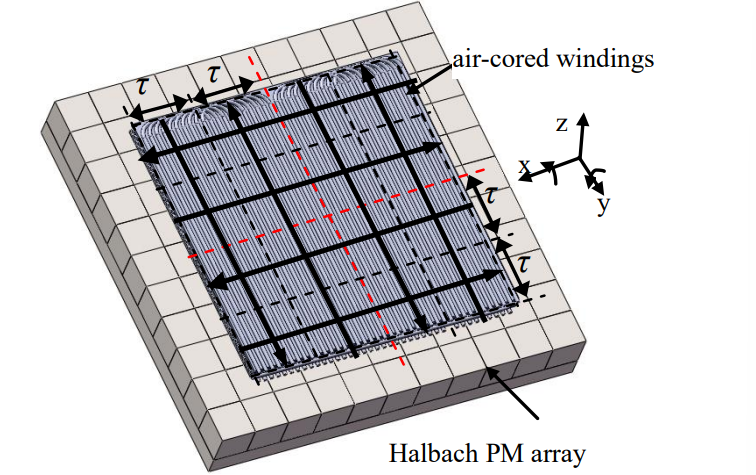
\includegraphics[width=0.5\textwidth]{Multilayer_Mover_Coil}}
%\hspace{2mm}
\subfloat[استفاده از سیم‌پیچ‌های یک لایه متعامد
\cite{RN14}]
{ \label{fig:Single_layer_Mover_Coil}
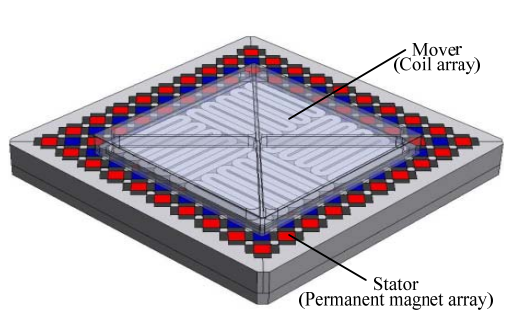
\includegraphics[width=0.5\textwidth]{Single_layer_Mover_Coil}}%
\caption{ساختار سیستم‌های MLPM با سیم‌پیچ‌های متحرک و آهنربای ثابت}
\label{fig:Moveing_Coil} %% label for entire figure
\end{figure}

با وجود اینکه این معماری امکان دستیابی به شناوری پایدار و حرکت با شش درجه آزادی را فراهم می‌کند، اما در کاربردهای عملی با محدودیت‌هایی مواجه است که بر عملکرد نهایی سیستم تأثیرگذار هستند. نخستین محدودیت، نیاز به تأمین انرژی الکتریکی برای سیم‌پیچ‌ها از طریق سیم‌های فیزیکی است که این امر به‌طور اجتناب‌ناپذیری ارتباط فیزیکی میان جسم متحرک و محیط اطراف را برقرار می‌سازد، در نتیجه حرکت آزادانه کامل جسم متحرک محدود می‌شود. دومین محدودیت، چالش خنک‌کاری سیم‌پیچ‌ها است که به دلیل ماهیت متحرک و معلق بودن آن‌ها، اجرای یک سیستم خنک‌کننده کارآمد دشوار خواهد بود. این مشکلات، نیاز به ارائه معماری جدیدی را آشکار می‌کند که بتواند این چالش‌ها را برطرف سازد.

\subsection{‌آهنرباهای متحرک و سیم‌پیچ‌های ثابت}

معماری دیگری که برای طراحی دستگاه‌های MLPM ارائه شده است، شامل قرار دادن سیم‌پیچ‌ها در بخش استاتور و استفاده از آهنرباهای دائمی در بخش متحرک می‌باشد. این ساختار نوین که در بسیاری از پژوهش‌ها مورد استفاده قرار گرفته، مشکلات معماری‌های پیشین مانند محدودیت جابه‌جایی متحرک ناشی از اتصالات فیزیکی و چالش‌های خنک‌کاری سیم‌پیچ‌ها را برطرف کرده و منجر به بهبود عملکرد کلی سیستم شده است.

در پژوهش 
\cite{RN7}
 استاتوری با چینش سیم‌پیچ‌ها مطابق با الگوی شاه‌ماهی
\LTRfootnote{Herringbone pattern}
 طراحی و پیاده‌سازی شده است. این طراحی امکان اعمال نیروی مغناطیسی به دو آهنربای دیسکی تعبیه‌شده در بخش متحرک را فراهم کرده است که دقتی در حدود 1 درجه در زوایای حرکت و 1 میلی‌متر در موقعیت متحرک به دست آورده است. در ادامه این پژوهش، ساختاری جدید برای بخش متحرک ارائه شده که شامل 6 آهنربای دیسکی با چینش کروی و فواصل ثابت می‌باشد. این طراحی توانسته است چرخش آزادانه متحرک را حول سه محور ممکن سازد 
\cite{RN39}.
شکل (
\ref{fig:Moving_Magnet_1})
همچنین در پژوهش 
\cite{RN62}
 نیز از این چینش سیم‌پیچ‌ها استفاده شده و مطابق با شبیه‌سازی‌های ارائه شده، مزیت آنان در ایجاد میدان مغناطیسی یکنواخت‌تر در نواحی کناری سیم‌پیچ‌ها نمایش داده شده است.

استفاده از سیم‌پیچ‌های سه‌فاز به‌جای تغذیه با جریان مستقیم، رویکردی است که در پژوهش 
\cite{RN24}
معرفی و اجرا شده است. در این ساختار، چهار آرایه از سیم‌پیچ‌های سه‌فاز، همان‌طور که در 
شکل (
\ref{fig:Moving_Magnet_2})
 نشان داده شده است، به‌گونه‌ای طراحی شده‌اند که نیروی مغناطیسی لازم را تولید کنند.

به ‌منظور کاهش هزینه‌ی محاسباتی در جابه‌جایی‌های طولانی، پژوهش 
\cite{RN32}
 ساختاری را ارائه کرده است که از دو مجموعه سیم‌پیچ‌ سه‌فاز و تک‌فاز تشکیل شده است. در این طراحی، کنترل حرکت در مسافت‌های طولانی توسط سیم‌پیچ‌های سه‌فاز انجام می‌پذیرد، در حالی که برای تنظیم دقیق موقعیت متحرک در صفحه، از سیم‌پیچ‌های تک‌فاز بهره برده می‌شود.
شکل (
\ref{fig:Moving_Magnet_3})

استفاده از سیم‌پیچ‌های ماژولار در طراحی استاتورهایی با چینش دوبعدی، رویکردی است که در دستگاه‌های MagTable و MagFloor از دانشگاه واترلو پیاده‌سازی شده است
\cite{RN8,RN30,RN10}
 در این طراحی، ماژول‌هایی از سیم‌پیچ‌های با سطح مقطع مربع به‌گونه‌ای طراحی شده‌اند که با قرار گرفتن در کنار یکدیگر، فضای کاری نامحدودی برای جابه‌جایی متحرک فراهم می‌کنند.(شکل
\ref{fig:Moving_Magnet_4})
 همچنین، پژوهش
\cite{RN8}
 نشان داده است که آهنرباهای با سطح مقطع مربع، در مقایسه با سیم‌پیچ‌های دایروی با جریان الکتریکی مشابه، می‌توانند شدت میدان مغناطیسی بیشتری ایجاد کنند، که این مزیت عملکرد کلی سیستم را بهبود می‌بخشد.

\begin{figure}[ht]
\centering 
\subfloat[الگوی شاه‌ماهی سیم‌پیچ‌ها
\cite{RN39}]
{ \label{fig:Moving_Magnet_1}
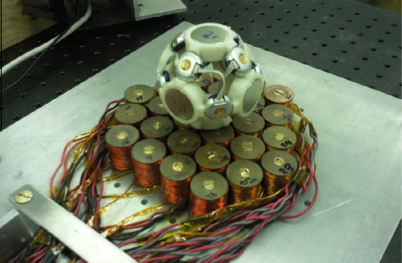
\includegraphics[width=0.45\textwidth]{Moving_Magnet_1}}
\hspace{2mm}
\subfloat[سیم‌پیچ‌های سه فاز
\cite{RN24}]
{ \label{fig:Moving_Magnet_2}
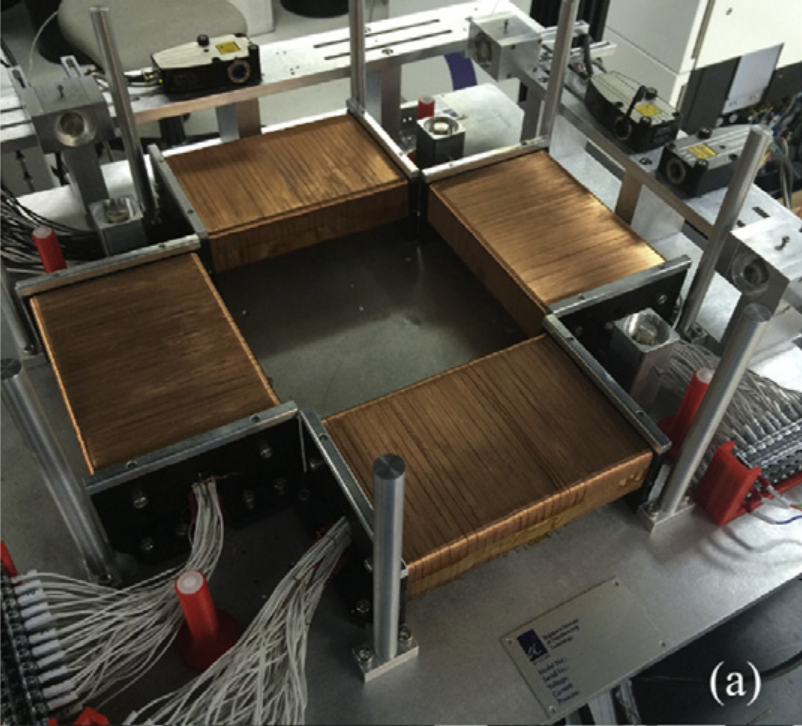
\includegraphics[width=0.45\textwidth]{Moving_Magnet_2}}
\\ % Newline to wrap the figures to the next row
\subfloat[ساختار دوگانه سیم‌پیچ‌ها
\cite{RN32}]
{ \label{fig:Moving_Magnet_3}
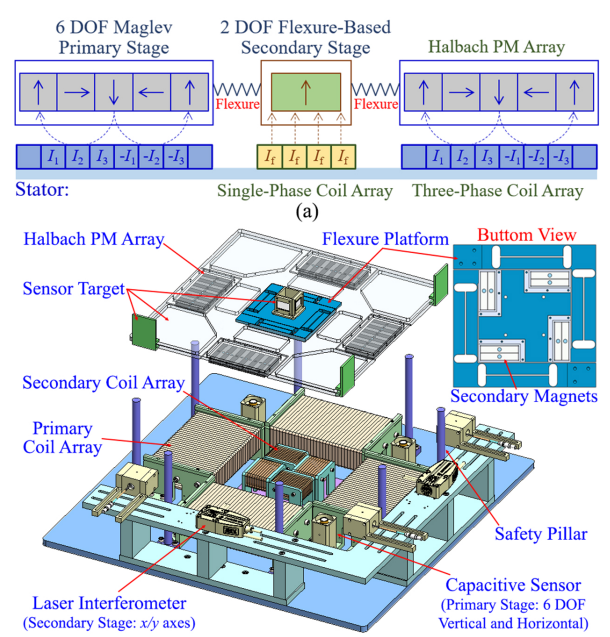
\includegraphics[width=0.45\textwidth]{Moving_Magnet_3}}
\hspace{2mm}
\subfloat[ساختار ماژولار سیم‌پیچ‌ها
\cite{RN10}]
{ \label{fig:Moving_Magnet_4}
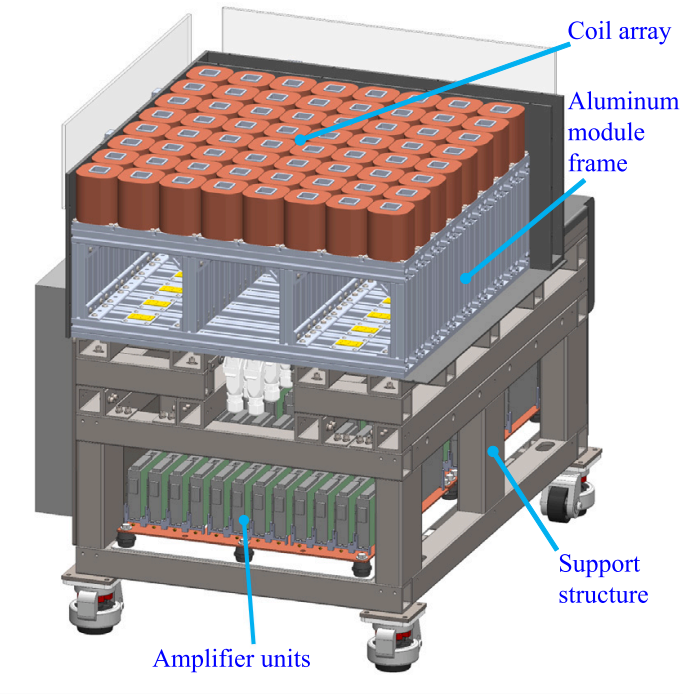
\includegraphics[width=0.45\textwidth]{Moving_Magnet_4}}
\label{fig:Moveing_Magnet} %% label for entire figure
\caption{ساختارهای آهنرباهای متحرک و سیم‌پیچ‌های ثابت}
\end{figure}








\section{مروری بر ادبیات موضوع}
در این قسمت باید به کارهای مشابه دیگران در گذشته اشاره کرد و وزن بیشتر این قسمت بهتر است به مقالات ژورنالی سال‌های اخیر (۲ تا ۳ سال) تخصیص داده شود. به نتایج کارهای دیگران با ذکر دقیق مراجع باید اشاره شده و جایگاه و تفاوت تحقیق شما نیز با کارهای دیگران مشخص شود. استفاده از مقالات ژورنال‌های معتبر در دو یا سه سال اخیر، می‌تواند به اعتبار کار شما بیافزاید.

.
.
.
.
.
.
.


\section{نتیجه‌گیری}
‌در نتیجه‌گیری آخر این فصل، با توجه به بررسی انجام شده بر روی مراجع تحقیق، بخش‌های قابل گسترش و تحقیق در آن حیطه و چشم‌اندازهای تحقیق مورد بررسی قرار می‌گیرند.	در برخی از تحقیقات، نتیجه نهایی فصل روش تحقیق، ارائهٔ یک چارچوب کار تحقیقی 
\lr{(research framework)}
است.
.
.
.
.
.